\taskpic{ На некоторых озёрах можно иногда наблюдать довольно
  необычное явление --- так называемые сейши (стоячие волны, при
  которых происходят колебания всей массы воды, причём поверхность
  водоёма наклоняется то в одну, то в другую сторону). Для создания
  модели сейшей используется прямоугольная ванночка. Толщина водяного
  слоя в ванне $h$, горизонтальная длина ванны $L$. Предположим, что
  поверхность воды вначале составляет небольшой угол с горизонтальной
  поверхностью. Тогда вода начинает качаться, то есть, поверхность
  воды остаётся ровной, но колеблется относительно горизонтальной
  поверхности. Постройте модель движения жидкости и найдите период
  колебаний сейшей $T$. Считайте, что $\delta \ll h$. 
 }
{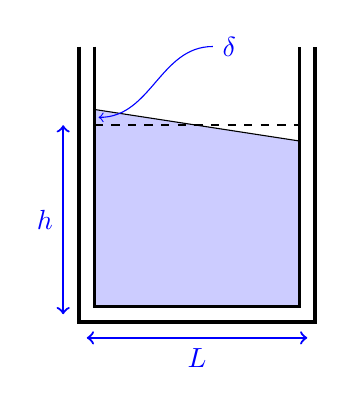
\begin{tikzpicture}
  \draw[fill=blue!20] (0.7,2.7) -- (0.7,0.2) -- (3.3,0.2) -- (3.3,2.3)
  -- (0.7,2.7);
  \draw[very thick] (0.5,3.5) -- (0.5,0) -- (3.5,0) --
  (3.5,3.5);
  \draw[very thick] (0.7,3.5) -- (0.7,0.2) -- (3.3,0.2) --
  (3.3,3.5);
  \draw[blue,thick,<->] (0.3,0.1) -- (0.3,2.5) node[midway,left]
  {$h$};
  \draw[blue,thick,<->] (0.6,-0.2) -- (3.4,-0.2) node[midway,below] {$L$};
  \draw[thick,dashed] (0.7,2.5) -- (3.3,2.5);
  \draw[blue,->] (2.2,3.5) node[right] {$\delta$} to[out=180,in=0](0.75,2.6);
  \end{tikzpicture}
}